\documentclass[10pt,a4paper]{article}
\usepackage[a4paper, margin=1.5cm]{geometry}
\usepackage{needspace}
\usepackage[nobottomtitles]{titlesec}
\usepackage{multicol}
\usepackage{xcolor}
\usepackage{fp}
\usepackage{xfp}
\usepackage{numprint}
\usepackage{siunitx}
\usepackage{enumitem}
\usepackage[version=4]{mhchem}
\usepackage{chemfig}
\usepackage{mol2chemfig}
\usepackage{WriteOnGrid}
\usepackage{frcursive}
\usepackage{csvsimple}%
\usepackage[francais,bloc]{automultiplechoice}

\DeclareSIUnit{\nothing}{\relax}

\FPseed=16

\baremeDefautS{e=0,v=0,b=1,m=-.25}
%\baremeDefautM{formula=(NBC>0 ? (NMC==0 ? 1:0):0)}

\graphicspath{ {./images/} }

\newenvironment{reponsesd}{
    \begin{multicols}{2}
    \begin{reponses} }{
    \end{reponses}
    \end{multicols}
}

% Sauvegarde l'ancienne définition de reponseshoriz
%\let\oldreponseshoriz\reponseshoriz
%\let\endoldreponseshoriz\endreponseshoriz

% Redéfinit reponseshoriz avec une taille de police réduite
%\renewenvironment{reponseshoriz}
%{
%    \scriptsize % ou \small, \scriptsize, etc.
%    \oldreponseshoriz
%}
%{
%    \endoldreponseshoriz
%}

\setlength{\columnseprule}{1pt}
\def\columnseprulecolor{\color{lightgray}}%

\let\oexplain\explain
\renewcommand{\explain}[1]{\oexplain{\textcolor{red}{#1}}}

\titleformat{\section}
  {\centering\hrule\vspace{2mm}}
  {\thesection}
  {1em}
  {}
  [\vspace{1mm}\hrule]

\titleformat{\subsection}
  {\em}
  {\thesubsection}
  {1em}
  {}

\newcommand{\sujet}{
\exemplaire{1}{%

\AMCsetFoot{\niveau{} \classe{} -- \prenom{}~\nom{} -- \thepage}
\AMCopenOpts{boxframerule=0pt,lineheight=0pt,width=0pt,boxframerulecol=white,
    dots=false,framerule=0pt,framerulecol=white}

%%% debut de l'en-tête des copies :
\begin{center}
\vfill
\noindent{\large \bf Classe de \niveau{}°\classe{}}

\vspace*{3mm}

{\Large\bf Évaluation sur table STL - Physique-Chime 05/01/2025}

\vfill
\namefield{\noindent{}\fbox{\vspace*{3mm}
         \Huge\bf\prenom{}~\nom{}\normalsize{}%
         \vspace*{3mm}
      }}
\end{center}
\vfill

\begin{center}
\textbf{Durée : une heure.}
\vspace*{5mm}

  Aucun document n'est autorisé.
  L'usage de la calculatrice est interdit.

  Les questions faisant apparaitre le symbole \multiSymbole{} peuvent
  présenter une ou plusieurs bonnes réponses. Les autres ont
  une unique bonne réponse.

  Des points négatifs seront affectés aux mauvaises réponses, \texbf{uniquement pour les QCM}. Pour les
  questions ouvertes (où vous écrivez la réponses dans les quadrillages), aucun point négatif ne sera appliqué.
  
  \vspace*{5mm}

  \textbf{IMPORTANT: Utilisez un crayon de papier bien noir pour cocher les cases, et une gomme
  pour effacer délicatement en cas d'erreur. Ne raturez pas les cases.
  Si vous effacez le pourtour de la case, ne le redessinez pas!}

  \vspace*{5mm}

  \textbf{IMPORTANT: Ne pas écrire dans les cases grisées!}

  \vspace*{5mm}

  Ne pas faire comme ceci (raturé, pas centré, trop pâle, ...):\\
  \includegraphics[width=4cm]{checkbox_bad.png}

  Mais comme cela (bien centré, bien foncé):\\
  \includegraphics[width=2cm]{checkbox_good.png}

  Si vous faites une erreur et que vous ne pouvez effacer, raturez la case bien ostensiblement.

\end{center}
\vspace{1ex}
\vfill
\pagebreak
%%% fin de l'en-tête

\restituegroupe{groupes}


\AMCassociation{\id}

	  } % End \exemplaire{1}{%
} % End \newcommand{\sujet}{


%%%%§§§§§§§§§§§§§§§§§§§§§§§§§§§§§§§§§
\newcommand{\allq}{}
\newcommand{\nball}[1]{#1}

\begin{document}
%%%Options
\AMCrandomseed{10}

\def\AMCformQuestion#1{{\sc Question #1 :}}

\setdefaultgroupmode{withoutreplacement}
%%% Fin Options

%%% elements
\input{q_01_simplenum.tex}

\element{power10}{
  \begin{question}{power101}
    Quelle est la valeur de \(10^3\)?
    \begin{reponses}
      \mauvaise{\numprint{100}}
      \mauvaise{\numprint{10000}}
      \mauvaise{\numprint{1000000}}
      \bonne{\numprint{1000}}
    \end{reponses}
    \explain{\(10^3 = 1000\)}
  \end{question}
}

\element{power10}{
  \begin{question}{power102}
    Quelle est la valeur de \(10^{-2}\)~?
    \begin{reponses}
      \mauvaise{\numprint{100}}
      \mauvaise{\numprint{-2}}
      \mauvaise{Un nombre imaginaire}
      \bonne{\numprint{0,01}}
    \end{reponses}
    \explain{\(10^{-2} = \frac{1}{100} = 0,01\)}
  \end{question}
}

\element{power10}{
  \begin{question}{power103}
    Comment écrire \numprint{0,001} sous forme de puissance de 10~?
    \begin{reponses}
      \mauvaise{$10^3$}
      \mauvaise{$-10^2$}
      \mauvaise{C'est impossible}
      \bonne{$10^{-3}$}
    \end{reponses}
    \explain{\(0,001 = \frac{1}{1000} = 10^{-3}\)}
  \end{question}
}

\element{power10}{
  \begin{question}{power104}
    Que vaut $\frac{10^2}{10^{-2}}$~?
    \begin{reponses}
      \mauvaise{$0$}
      \mauvaise{$1$}
      \mauvaise{Indéfini}
      \bonne{$10^4$}
    \end{reponses}
    \explain{\(\frac{10^2}{10^{-2}} = 10^2 \times 10^{2} = 10^4\)}
  \end{question}
}

\element{power10}{
  \begin{question}{power105}
    Quelle est la valeur de $10^4$?
    \begin{reponses}
      \mauvaise{\numprint{100}}
      \mauvaise{\numprint{1000}}
      \mauvaise{\numprint{1000000}}
      \bonne{\numprint{10000}}
    \end{reponses}
    \explain{$10^4 = 10000$}
  \end{question}
}

\element{power10}{
  \begin{question}{power106}
    Quelle est la valeur de $10^{-3}$~?
    \begin{reponses}
      \mauvaise{\numprint{1000}}
      \mauvaise{\numprint{-3}}
      \mauvaise{\numprint{0,01}}
      \bonne{\numprint{0,001}}
    \end{reponses}
    \explain{$10^{-3} = \frac{1}{1000} = 0,001$}
  \end{question}
}

\element{power10}{
  \begin{question}{power107}
    Comment écrire \numprint{0,0001} sous forme de puissance de 10~?
    \begin{reponses}
      \mauvaise{$10^4$}
      \mauvaise{$-10^3$}
      \mauvaise{$10^{-3}$}
      \bonne{$10^{-4}$}
    \end{reponses}
    \explain{\numprint{0,0001} = $10^{-4}$}
  \end{question}
}

\element{power10}{
  \begin{question}{power108}
    Que vaut $\frac{10^3}{10^{-2}}$~?
    \begin{reponseshoriz}
      \mauvaise{$0$}
      \mauvaise{$1$}
      \mauvaise{$10^4$}
      \bonne{$10^5$}
    \end{reponseshoriz}
    \explain{$\frac{10^3}{10^{-2}} = 10^3 \times 10^{2} = 10^5$}
  \end{question}
}


\element{psi}{
  \begin{question}{psi1}
    Quel est le symbole du préfixe représentant $10^3$~?
    \begin{reponseshoriz}
      \mauvaise{\si{\mega\nothing}}
      \mauvaise{\si{\giga\nothing}}
      \mauvaise{\si{\tera\nothing}}
      \bonne{\si{\kilo\nothing}}
    \end{reponseshoriz}
    \explain{Le symbole est $\si{\kilo\nothing} = 10^3$, $\si{\mega\nothing} = 10^6$, $\si{\giga\nothing} = 10^9$ 
    et $\si{\tera\nothing} = 10^{12}$}
  \end{question}
}

\element{psi}{
  \begin{question}{psi2}
    Quelle est la valeur de \qty{1}{\micro\second}~?
    \begin{reponses}
      \mauvaise{\qty{1 e6}{\second}}
      \mauvaise{\qty{1 e-3}{\second}}
      \mauvaise{\qty{1 e3}{\second}}
      \bonne{\qty{1 e-6}{\second}}
    \end{reponses}
    \explain{La valeur de \qty{1}{\micro\second} est \qty{1 e-6}{\second}, $\qty{1 e6}{\second} = \qty{1}{\mega\second}$, 
    $\qty{1 e-3}{\second} = \qty{1}{\milli\second}$ et $\qty{1 e3}{\second} = \qty{1}{\kilo\second}$}
  \end{question}
}

\element{psi}{
  \begin{question}{psi3}
    Quel préfixe correspond à $10^{-6}$~?
    \begin{reponseshoriz}
      \mauvaise{\si{\milli\nothing}}
      \mauvaise{\si{\kilo\nothing}}
      \mauvaise{\si{\nano\nothing}}
      \bonne{\si{\micro\nothing}}
    \end{reponseshoriz}
    \explain{Le préfixe est $\si{\micro\nothing} = 10^{-6}$, $\si{\milli\nothing} = 10^{-3}$, 
    $\si{\nano\nothing} = 10^{-9}$ et $\si{\kilo\nothing} = 10^3$}
  \end{question}
}

\element{psi}{
  \begin{question}{psi4}
    Quelle quantité en unités de base correspond à \qty{5}{\kilo\metre}~?
    \begin{reponses}
      \mauvaise{\qty{5}{\metre}}
      \mauvaise{\qty{5}{\milli\metre}}
      \mauvaise{\qty{500}{\metre}}
      \bonne{\qty{5000}{\metre}}
    \end{reponses}
    \explain{$5 \, \si{\kilo\metre} = 5 000 \, \text{m}$, car $\si{\kilo\nothing} = 10^3$}
  \end{question}
}

\input{q_04_atoms.tex}
% symboles chimiques
\element{symchim}{
  \begin{question}{symchim1}
    Quel est le symbole chimique du carbone~?
    \begin{reponseshoriz}
      \mauvaise{\ce{H}}
      \mauvaise{\ce{O}}
      \mauvaise{\ce{N}}
      \bonne{\ce{C}}
    \end{reponseshoriz}
    \explain{Le symbole chimique du carbone est \ce{C}.}
  \end{question}
}

\element{symchim}{
  \begin{question}{symchim2}
    Quel est le symbole chimique de l'oxygène~?
    \begin{reponseshoriz}
      \mauvaise{\ce{C}}
      \mauvaise{\ce{H}}
      \mauvaise{\ce{N}}
      \bonne{\ce{O}}
    \end{reponseshoriz}
    \explain{Le symbole chimique de l'oxygène est \ce{O}.}
  \end{question}
}

\element{symchim}{
  \begin{question}{symchim3}
    Quel est le symbole chimique de l'azote~?
    \begin{reponseshoriz}
      \mauvaise{\ce{C}}
      \mauvaise{\ce{H}}
      \mauvaise{\ce{O}}
      \bonne{\ce{N}}
    \end{reponseshoriz}
    \explain{Le symbole chimique de l'azote est \ce{N}.}
  \end{question}
}

\element{symchim}{
  \begin{question}{symchim4}
    Quel est le symbole chimique de l'hydrogène~?
    \begin{reponseshoriz}
      \mauvaise{\ce{C}}
      \mauvaise{\ce{O}}
      \mauvaise{\ce{N}}
      \bonne{\ce{H}}
    \end{reponseshoriz}
    \explain{Le symbole chimique de l'hydrogène est \ce{H}.}
  \end{question}
}

% Notation des symboles chimiques
\element{symchim}{
  \begin{question}{symchim5}
    Dans le symbole \ce{^A_ZX}, qu'est-ce que représente Z~?
    \begin{reponses}
      \mauvaise{Le nombre de neutrons}
      \mauvaise{Le nombre de nucléons}
      \mauvaise{Le numéro de masse}
      \bonne{Le nombre de protons}
    \end{reponses}
    \explain{Dans le symbole \ce{^A_ZX}, Z représente le nombre de protons, qui correspond au numéro atomique de l'élément.}
  \end{question}
}

\element{symchim}{
  \begin{question}{symchim6}
    Dans le symbole \ce{^A_ZX}, qu'est-ce que représente A~?
    \begin{reponses}
      \mauvaise{Le nombre de protons}
      \mauvaise{Le nombre de neutrons}
      \mauvaise{La charge électrique de l'atome}
      \bonne{Le nombre de nucléons}
    \end{reponses}
    \explain{Dans le symbole \ce{^A_ZX}, A représente le nombre total de nucléons, c'est-à-dire la somme des protons et des neutrons.}
  \end{question}
}

\element{symchim}{
  \begin{question}{symchim7}
    Dans le symbole \ce{^A_ZX}, comment peut-on déterminer le nombre de neutrons~?
    \begin{reponses}
      \mauvaise{En additionnant Z et A}
      \mauvaise{En soustrayant A de Z (Z-A)}
      \mauvaise{En multipliant Z par A}
      \bonne{En soustrayant Z de A (A-Z)}
    \end{reponses}
    \explain{Le nombre de neutrons est obtenu en soustrayant le nombre de protons (Z) du nombre total de nucléons (A).}
  \end{question}
}

\element{symchim}{
  \begin{question}{symchim8}
    Dans le symbole \ce{^14_6C}, combien y a-t-il de neutrons~?
    \begin{reponseshoriz}
      \mauvaise{6}
      \mauvaise{10}
      \mauvaise{12}
      \bonne{8}
    \end{reponseshoriz}
    \explain{Le nombre de protons Z est 6, et le nombre de nucléons A est 14. Donc, le nombre de neutrons est 14 - 6 = 8.}
  \end{question}
}

\input{q_alcans.tex}
\input{q_alcools.tex}
\input{q_groups.tex}
\input{q_nomencla.tex}
\input{q_isors.tex}
\input{q_isoze.tex}
%\begin{questionmult}{acidbenzo1}
    Entourer et nommer le groupe caractéristique présents dans la formule topologique de l'acide benzoïque ci-dessous.\\
        \centering\chemfig{OH-[:120,,1](=[:60]O)-[:180]=_[:240]-[:180]=_[:120]-[:60]=_(-[:300])}\\
    \AMCOpen{}{
        \mauvaise[F]{NA}\scoring{b=0}
        \mauvaise[X]{Faux}\scoring{b=-1}
        \bonne[I]{Groupe identifié}\scoring{b=.5}
        \bonne[N]{Groupe nommé}\scoring{b=.5}
    }
    \explain{Le groupes caractéristique est le groupe carboxyle (–COOH)}
\end{questionmult}

\begin{question}{acidbenzo2}
    Écrire la formule topologique de l’ion benzoate, base conjuguée de l’acide benzoïque.\\
    \begin{EnvQuadrillage}[NbCarreaux=20x4,Grille=Seyes,Marge=1]
    \end{EnvQuadrillage}
    \AMCOpen{}{
        \mauvaise[F]{NA}\scoring{b=0}
        \mauvaise[X]{Faux}\scoring{b=-1}
        \mauvaise[B]{\approx}\scoring{b=.5}
        \bonne[A]{OK}\scoring{b=1}
    }
    \explain{
    La formule topologique de l’ion benzoate est :
    mcfright{O}{^{\mcfminus}}-[:210](=[:150]O)-[:270]=^[:210]-[:270]=^[:330]%
-[:30]=^[:90](-[:150])}
\end{question}

\begin{question}{acidbenzo3}
    Représenter le diagramme de prédominance du couple acide benzoïque/ion benzoate.\\
    \begin{EnvQuadrillage}[NbCarreaux=20x4,Grille=Seyes,Marge=1]
    \end{EnvQuadrillage}
    \AMCOpen{}{
        \mauvaise[F]{NA}\scoring{b=0}
        \mauvaise[X]{Faux}\scoring{b=-1}
        \mauvaise[B]{\approx}\scoring{b=1}
        \bonne[A]{OK}\scoring{b=2}
    }
    \explain{
    Le diagramme de prédominance du couple acide benzoïque/ion benzoate doit montrer que :
    - À un pH inférieur au pKa (4,2), l'acide benzoïque (\ce{C6H5COOH}) est prédominant.
    - À un pH supérieur au pKa (4,2), l'ion benzoate (\ce{C6H5COO-}) est prédominant.
    }
\end{question}

\subsection{Expériences}

Dans un premier temps, on réalise deux expériences permettant de mettre en évidence les propriétés de l’acide
benzoïque et de l’ion benzoate :
\begin{itemize}
\item Expérience (1) : Dans un tube à essais contenant une solution de benzoate de sodium, on ajoute quelques
gouttes d’acide chlorhydrique concentré. On observe qu’un solide blanc apparaît.
\item Expérience (2) : Dans un tube à essais contenant une solution de soude concentrée, on ajoute de l’acide
benzoïque solide. On observe que le solide introduit disparaît.
\end{itemize}

\begin{questionmult}{acidbenzo4}
    On donne l'équation chimique suivante :\\
    \ce{C6H5COO^-_{(aq)} + H3O^+_{(aq)} -> C6H5COOH_{(aq)} + H2O_{(l)}}\\
    La réaction qui correspond à l'équation ci-dessus modélise une transformation chimique ayant lieu lors de l'une 
    des expériences précédentes. Indiquer, en justifiant la réponse, s'il s'agit de l'expérience (1) ou de l'expérience (2).
    \begin{EnvQuadrillage}[NbCarreaux=20x6,Grille=Seyes,Marge=1]
    \end{EnvQuadrillage}
    \AMCOpen{}{
        \mauvaise[F]{NA}\scoring{b=0}
        \mauvaise[X]{Faux}\scoring{b=-1}
        \bonne[P]{Expérience identifiée}\scoring{b=0.5}
        \bonne[C]{Justification correcte}\scoring{b=0.5}
    }
    \explain{
    Il s'agit de l'expérience (1). Les réactifs sont l'ion benzoate et l'ion oxonium, qui correspondent aux réactifs de 
    l'expérience 1, les ions oxonium étant apportés par la solution d'acide chlorhydrique.
    }
\end{questionmult}

L’étiquette d’une boisson gazeuse indique qu’elle contient du benzoate de sodium comme conservateur alimentaire,
entre autres, et on souhaite vérifier cette indication. On réalise pour cela une extraction liquide-liquide.
On suit le protocole expérimental suivant :

\begin{enumerate}
    \item Verser 500 mL de boisson dans un grand bécher.
    \item Ajouter de l’acide chlorhydrique jusqu’à amener le pH à environ 2.
    \item Ajouter alors 40 mL d’éther éthylique, agiter et laisser reposer.
    \item Transvaser l’ensemble dans une ampoule à décanter.
    \item Agiter vigoureusement pendant deux minutes en prenant soin de dégazer régulièrement pour éviter toute surpression.
    \item Laisser décanter.
    \item Récupérer la phase aqueuse S dans un bécher et la phase organique dans un erlenmeyer.
\end{enumerate}


\begin{questionmult}{acidbenzo5}
    Préciser ce qu'il se passe lors de l'étape 2 du protocole.
    \begin{EnvQuadrillage}[NbCarreaux=20x5,Grille=Seyes,Marge=1]
    \end{EnvQuadrillage}
    \AMCOpen{}{
        \mauvaise[F]{NA}\scoring{b=0}
        \mauvaise[X]{Faux}\scoring{b=-1}
        \bonne[A]{Eq}\scoring{b=.5}
        \bonne[B]{Prd}\scoring{b=.5}
    }
    \explain{
    Lors de l'étape 2 du protocole, l'ion benzoate se transforme en acide benzoïque suite à l'ajout d'acide chlorhydrique. 
    En effet, on ajoute l'acide chlorhydrique jusqu'à pH = 2, c'est-à-dire un pH inférieur au pKa du couple. 
    Il s'agit donc de la zone de prédominance de l'acide benzoïque.
    }
\end{questionmult}

\begin{question}{acidbenzo6}
    À l'aide des données, expliquer pourquoi l'éther éthylique constitue un solvant extracteur plus adapté que 
    l'éthanol lors de la réalisation de l'étape 3 du protocole.
    \begin{EnvQuadrillage}[NbCarreaux=20x6,Grille=Seyes,Marge=1]
    \end{EnvQuadrillage}
    \AMCOpen{}{
        \mauvaise[F]{NA}\scoring{b=0}
        \mauvaise[X]{Faux}\scoring{b=-1}
        \mauvaise[C]{\approx}\scoring{b=.5}
        \bonne[C]{OK}\scoring{b=1}
    }
    \explain{
    L'éther éthylique est non miscible à l'eau et l'acide benzoïque y est très soluble, contrairement à l'éthanol qui 
    est miscible à l'eau. Cela en fait un solvant extracteur plus adapté.
    }
\end{question}

\begin{questionmult}{acidbenzo7}
    Compléter le schéma ci-dessous, en justifiant, à l'aide des données, la nature 
    et la position des différentes phases dans l'ampoule à décanter à l'issue de l'étape 6 du protocole.

    \begin{center}
        \begin{minipage}[t]{0.4\textwidth}
            \centering
            \includegraphics[height=5cm, keepaspectratio]{images/ste5_ampoule.png}
        \end{minipage}%
        \begin{minipage}[t]{0.6\textwidth}
            \begin{EnvQuadrillage}[NbCarreaux=12x6, Grille=Seyes,Marge=1]
            \end{EnvQuadrillage}
        \end{minipage}
    \end{center}

    \AMCOpen{}{
        \mauvaise[F]{NA}\scoring{b=0}
        \mauvaise[X]{Faux}\scoring{b=-1}
        \bonne[C]{ScBuoy}\scoring{b=.5}
        \bonne[C]{ScAcd}\scoring{b=.5}
        \bonne[C]{XpBuoy}\scoring{b=.5}
        \bonne[C]{Ovl}\scoring{b=.5}
   }
    \explain{
    L'éther éthylique (densité = 0,71) est moins dense que l'eau (densité = 1,0). La phase organique (éther) 
    constitue donc la phase supérieure et la phase aqueuse, la phase inférieure.
    }
\end{questionmult}

\begin{question}{acidbenzo8}
    Après évaporation du solvant extracteur, il reste une masse \( m = 10,0 \) mg de solide blanc. Proposer 
    une méthode expérimentale permettant de vérifier que ce solide blanc est bien de l'acide benzoïque.
    \begin{EnvQuadrillage}[NbCarreaux=20x4,Grille=Seyes,Marge=1]
    \end{EnvQuadrillage}
    \AMCOpen{}{
        \mauvaise[F]{NA}\scoring{b=0}
        \mauvaise[X]{Faux}\scoring{b=-1}
        \bonne[B]{\approx}\scoring{b=.5}
        \bonne[A]{OK}\scoring{b=1}
   }
    \explain{
    On peut mesurer son point de fusion au banc Kofler et vérifier qu'il est bien de \(122,4^\circ C\). Une 
    chromatographie sur couche mince ou un spectre infra-rouge/RMN peuvent aussi être réalisés pour confirmation.
    }
\end{question}

\begin{questionmult}{acidbenzo9}
    Sachant que la concentration $C$ en quantité de matière totale théorique d'ions benzoate dans cette 
    boisson est égale à \qty{4.0e-4}{\mol\per\litre}, montrer que la masse théorique d'acide 
    benzoïque que l'on devrait obtenir à l'issue de l'extraction est égale à \qty{24}{\mg}.

    \begin{EnvQuadrillage}[NbCarreaux=20x8,Grille=Seyes,Marge=1]
    \end{EnvQuadrillage}

    \AMCOpen{}{
        \mauvaise[F]{NA}\scoring{b=0}
        \mauvaise[X]{Faux}\scoring{b=-1}
        \bonne[C]{Idée}\scoring{b=.5}
        \bonne[B]{Forml}\scoring{b=.5}
        \bonne[A]{Nb}\scoring{b=.5}
        \bonne[A]{Ovl}\scoring{b=.5}
    }

    \explain{
    La masse théorique d'acide benzoïque est calculée comme suit :
    \[
    m = C \times V \times M = \SI{4.0e-4}{\mol\per\litre} \times \SI{0.5}{\litre} \times \SI{122}{\gram\per\mol} = \SI{24}{\milligram}
    \]
    }
\end{questionmult}

\begin{questionmult}{acidbenzo10}
    Le rendement d'une extraction étant défini comme le rapport de la masse de substance réellement extraite sur la 
    masse théorique de substance que l'on aurait pu extraire, calculer le rendement de cette extraction et 
    l'exprimer en pourcentage. Commenter ce résultat.
    \begin{EnvQuadrillage}[NbCarreaux=20x4,Grille=Seyes,Marge=1]
    \end{EnvQuadrillage}
    \AMCOpen{}{
        \mauvaise[F]{NA}\scoring{b=0}
        \mauvaise[X]{Faux}\scoring{b=-1}
        \bonne[C]{Idée}\scoring{b=.5}
        \bonne[B]{Forml}\scoring{b=.5}
        \bonne[A]{Nb}\scoring{b=.5}
        \bonne[A]{Ovl}\scoring{b=.5}
    }
    \explain{
    Le rendement est calculé comme suit :
    \[
    \eta = \frac{10,0}{24} \times 100 = 41,7\%
    \]
    Ce rendement est relativement faible. Pour l'améliorer, il faudrait extraire une deuxième fois la phase aqueuse avec
     40 mL d'éther éthylique puis rassembler les phases organiques.
    }
\end{questionmult}


%%% fin des elements
\element{groupes}{
\section{Rappels simples sur des notions mathématiques et physiques}
\begin{multicols}{2}
\insertgroup[2]{simplenum}
\insertgroup[2]{power10}
\insertgroup[2]{psi}
\insertgroup[2]{atoms}
\insertgroup[2]{symchim}
\end{multicols}

\section{Nomenclature des alcanes}
\begin{multicols}{2}
\insertgroup[2]{falcans}
\insertgroup[2]{alcans}
\insertgroup[2]{alcools}
\insertgroup[2]{groups}
\insertgroup[2]{nomencla}
\insertgroup[2]{isors}
\insertgroup[2]{isoze}
\end{multicols}

\begin{questionmult}{acidbenzo1}
    Entourer et nommer le groupe caractéristique présents dans la formule topologique de l'acide benzoïque ci-dessous.\\
        \centering\chemfig{OH-[:120,,1](=[:60]O)-[:180]=_[:240]-[:180]=_[:120]-[:60]=_(-[:300])}\\
    \AMCOpen{}{
        \mauvaise[F]{NA}\scoring{b=0}
        \mauvaise[X]{Faux}\scoring{b=-1}
        \bonne[I]{Groupe identifié}\scoring{b=.5}
        \bonne[N]{Groupe nommé}\scoring{b=.5}
    }
    \explain{Le groupes caractéristique est le groupe carboxyle (–COOH)}
\end{questionmult}

\begin{question}{acidbenzo2}
    Écrire la formule topologique de l’ion benzoate, base conjuguée de l’acide benzoïque.\\
    \begin{EnvQuadrillage}[NbCarreaux=20x4,Grille=Seyes,Marge=1]
    \end{EnvQuadrillage}
    \AMCOpen{}{
        \mauvaise[F]{NA}\scoring{b=0}
        \mauvaise[X]{Faux}\scoring{b=-1}
        \mauvaise[B]{\approx}\scoring{b=.5}
        \bonne[A]{OK}\scoring{b=1}
    }
    \explain{
    La formule topologique de l’ion benzoate est :
    mcfright{O}{^{\mcfminus}}-[:210](=[:150]O)-[:270]=^[:210]-[:270]=^[:330]%
-[:30]=^[:90](-[:150])}
\end{question}

\begin{question}{acidbenzo3}
    Représenter le diagramme de prédominance du couple acide benzoïque/ion benzoate.\\
    \begin{EnvQuadrillage}[NbCarreaux=20x4,Grille=Seyes,Marge=1]
    \end{EnvQuadrillage}
    \AMCOpen{}{
        \mauvaise[F]{NA}\scoring{b=0}
        \mauvaise[X]{Faux}\scoring{b=-1}
        \mauvaise[B]{\approx}\scoring{b=1}
        \bonne[A]{OK}\scoring{b=2}
    }
    \explain{
    Le diagramme de prédominance du couple acide benzoïque/ion benzoate doit montrer que :
    - À un pH inférieur au pKa (4,2), l'acide benzoïque (\ce{C6H5COOH}) est prédominant.
    - À un pH supérieur au pKa (4,2), l'ion benzoate (\ce{C6H5COO-}) est prédominant.
    }
\end{question}

\subsection{Expériences}

Dans un premier temps, on réalise deux expériences permettant de mettre en évidence les propriétés de l’acide
benzoïque et de l’ion benzoate :
\begin{itemize}
\item Expérience (1) : Dans un tube à essais contenant une solution de benzoate de sodium, on ajoute quelques
gouttes d’acide chlorhydrique concentré. On observe qu’un solide blanc apparaît.
\item Expérience (2) : Dans un tube à essais contenant une solution de soude concentrée, on ajoute de l’acide
benzoïque solide. On observe que le solide introduit disparaît.
\end{itemize}

\begin{questionmult}{acidbenzo4}
    On donne l'équation chimique suivante :\\
    \ce{C6H5COO^-_{(aq)} + H3O^+_{(aq)} -> C6H5COOH_{(aq)} + H2O_{(l)}}\\
    La réaction qui correspond à l'équation ci-dessus modélise une transformation chimique ayant lieu lors de l'une 
    des expériences précédentes. Indiquer, en justifiant la réponse, s'il s'agit de l'expérience (1) ou de l'expérience (2).
    \begin{EnvQuadrillage}[NbCarreaux=20x6,Grille=Seyes,Marge=1]
    \end{EnvQuadrillage}
    \AMCOpen{}{
        \mauvaise[F]{NA}\scoring{b=0}
        \mauvaise[X]{Faux}\scoring{b=-1}
        \bonne[P]{Expérience identifiée}\scoring{b=0.5}
        \bonne[C]{Justification correcte}\scoring{b=0.5}
    }
    \explain{
    Il s'agit de l'expérience (1). Les réactifs sont l'ion benzoate et l'ion oxonium, qui correspondent aux réactifs de 
    l'expérience 1, les ions oxonium étant apportés par la solution d'acide chlorhydrique.
    }
\end{questionmult}

L’étiquette d’une boisson gazeuse indique qu’elle contient du benzoate de sodium comme conservateur alimentaire,
entre autres, et on souhaite vérifier cette indication. On réalise pour cela une extraction liquide-liquide.
On suit le protocole expérimental suivant :

\begin{enumerate}
    \item Verser 500 mL de boisson dans un grand bécher.
    \item Ajouter de l’acide chlorhydrique jusqu’à amener le pH à environ 2.
    \item Ajouter alors 40 mL d’éther éthylique, agiter et laisser reposer.
    \item Transvaser l’ensemble dans une ampoule à décanter.
    \item Agiter vigoureusement pendant deux minutes en prenant soin de dégazer régulièrement pour éviter toute surpression.
    \item Laisser décanter.
    \item Récupérer la phase aqueuse S dans un bécher et la phase organique dans un erlenmeyer.
\end{enumerate}


\begin{questionmult}{acidbenzo5}
    Préciser ce qu'il se passe lors de l'étape 2 du protocole.
    \begin{EnvQuadrillage}[NbCarreaux=20x5,Grille=Seyes,Marge=1]
    \end{EnvQuadrillage}
    \AMCOpen{}{
        \mauvaise[F]{NA}\scoring{b=0}
        \mauvaise[X]{Faux}\scoring{b=-1}
        \bonne[A]{Eq}\scoring{b=.5}
        \bonne[B]{Prd}\scoring{b=.5}
    }
    \explain{
    Lors de l'étape 2 du protocole, l'ion benzoate se transforme en acide benzoïque suite à l'ajout d'acide chlorhydrique. 
    En effet, on ajoute l'acide chlorhydrique jusqu'à pH = 2, c'est-à-dire un pH inférieur au pKa du couple. 
    Il s'agit donc de la zone de prédominance de l'acide benzoïque.
    }
\end{questionmult}

\begin{question}{acidbenzo6}
    À l'aide des données, expliquer pourquoi l'éther éthylique constitue un solvant extracteur plus adapté que 
    l'éthanol lors de la réalisation de l'étape 3 du protocole.
    \begin{EnvQuadrillage}[NbCarreaux=20x6,Grille=Seyes,Marge=1]
    \end{EnvQuadrillage}
    \AMCOpen{}{
        \mauvaise[F]{NA}\scoring{b=0}
        \mauvaise[X]{Faux}\scoring{b=-1}
        \mauvaise[C]{\approx}\scoring{b=.5}
        \bonne[C]{OK}\scoring{b=1}
    }
    \explain{
    L'éther éthylique est non miscible à l'eau et l'acide benzoïque y est très soluble, contrairement à l'éthanol qui 
    est miscible à l'eau. Cela en fait un solvant extracteur plus adapté.
    }
\end{question}

\begin{questionmult}{acidbenzo7}
    Compléter le schéma ci-dessous, en justifiant, à l'aide des données, la nature 
    et la position des différentes phases dans l'ampoule à décanter à l'issue de l'étape 6 du protocole.

    \begin{center}
        \begin{minipage}[t]{0.4\textwidth}
            \centering
            \includegraphics[height=5cm, keepaspectratio]{images/ste5_ampoule.png}
        \end{minipage}%
        \begin{minipage}[t]{0.6\textwidth}
            \begin{EnvQuadrillage}[NbCarreaux=12x6, Grille=Seyes,Marge=1]
            \end{EnvQuadrillage}
        \end{minipage}
    \end{center}

    \AMCOpen{}{
        \mauvaise[F]{NA}\scoring{b=0}
        \mauvaise[X]{Faux}\scoring{b=-1}
        \bonne[C]{ScBuoy}\scoring{b=.5}
        \bonne[C]{ScAcd}\scoring{b=.5}
        \bonne[C]{XpBuoy}\scoring{b=.5}
        \bonne[C]{Ovl}\scoring{b=.5}
   }
    \explain{
    L'éther éthylique (densité = 0,71) est moins dense que l'eau (densité = 1,0). La phase organique (éther) 
    constitue donc la phase supérieure et la phase aqueuse, la phase inférieure.
    }
\end{questionmult}

\begin{question}{acidbenzo8}
    Après évaporation du solvant extracteur, il reste une masse \( m = 10,0 \) mg de solide blanc. Proposer 
    une méthode expérimentale permettant de vérifier que ce solide blanc est bien de l'acide benzoïque.
    \begin{EnvQuadrillage}[NbCarreaux=20x4,Grille=Seyes,Marge=1]
    \end{EnvQuadrillage}
    \AMCOpen{}{
        \mauvaise[F]{NA}\scoring{b=0}
        \mauvaise[X]{Faux}\scoring{b=-1}
        \bonne[B]{\approx}\scoring{b=.5}
        \bonne[A]{OK}\scoring{b=1}
   }
    \explain{
    On peut mesurer son point de fusion au banc Kofler et vérifier qu'il est bien de \(122,4^\circ C\). Une 
    chromatographie sur couche mince ou un spectre infra-rouge/RMN peuvent aussi être réalisés pour confirmation.
    }
\end{question}

\begin{questionmult}{acidbenzo9}
    Sachant que la concentration $C$ en quantité de matière totale théorique d'ions benzoate dans cette 
    boisson est égale à \qty{4.0e-4}{\mol\per\litre}, montrer que la masse théorique d'acide 
    benzoïque que l'on devrait obtenir à l'issue de l'extraction est égale à \qty{24}{\mg}.

    \begin{EnvQuadrillage}[NbCarreaux=20x8,Grille=Seyes,Marge=1]
    \end{EnvQuadrillage}

    \AMCOpen{}{
        \mauvaise[F]{NA}\scoring{b=0}
        \mauvaise[X]{Faux}\scoring{b=-1}
        \bonne[C]{Idée}\scoring{b=.5}
        \bonne[B]{Forml}\scoring{b=.5}
        \bonne[A]{Nb}\scoring{b=.5}
        \bonne[A]{Ovl}\scoring{b=.5}
    }

    \explain{
    La masse théorique d'acide benzoïque est calculée comme suit :
    \[
    m = C \times V \times M = \SI{4.0e-4}{\mol\per\litre} \times \SI{0.5}{\litre} \times \SI{122}{\gram\per\mol} = \SI{24}{\milligram}
    \]
    }
\end{questionmult}

\begin{questionmult}{acidbenzo10}
    Le rendement d'une extraction étant défini comme le rapport de la masse de substance réellement extraite sur la 
    masse théorique de substance que l'on aurait pu extraire, calculer le rendement de cette extraction et 
    l'exprimer en pourcentage. Commenter ce résultat.
    \begin{EnvQuadrillage}[NbCarreaux=20x4,Grille=Seyes,Marge=1]
    \end{EnvQuadrillage}
    \AMCOpen{}{
        \mauvaise[F]{NA}\scoring{b=0}
        \mauvaise[X]{Faux}\scoring{b=-1}
        \bonne[C]{Idée}\scoring{b=.5}
        \bonne[B]{Forml}\scoring{b=.5}
        \bonne[A]{Nb}\scoring{b=.5}
        \bonne[A]{Ovl}\scoring{b=.5}
    }
    \explain{
    Le rendement est calculé comme suit :
    \[
    \eta = \frac{10,0}{24} \times 100 = 41,7\%
    \]
    Ce rendement est relativement faible. Pour l'améliorer, il faudrait extraire une deuxième fois la phase aqueuse avec
     40 mL d'éther éthylique puis rassembler les phases organiques.
    }
\end{questionmult}


\section{Stéréochimie et réactions acido-basiques de l'ibuprofène}
\textbf{Source du sujet :} Baccalauréat de mars 2021

\subsection{Introduction}
Au XIX\textsuperscript{e} siècle, on utilisait déjà des principes actifs chiraux comme la morphine, administrée comme
anti-douleur. Malgré les idées énoncées par Pasteur à la fin du XIXtextsuperscript{e} siècle, les chimistes ont
mis beaucoup de temps pour comprendre que la chiralité pouvait avoir un impact considérable sur
les organismes vivants. Cette prise de conscience a eu lieu dans les années 1960 avec le drame de
la thalidomide, médicament qui fut administré aux femmes enceintes comme anti-vomitif, et qui
provoqua chez les nouveau-nés de graves malformations. On connaît aujourd'hui la raison de ce drame~:
alors que l'énantiomère $R$ est bien anti-vomitif, l'énantiomère $S$ est tératogène*.

L'ibuprofène est connu pour avoir un effet biologique anti-inflammatoire et antipyrétique sous sa
forme $S$ et sans effet thérapeutique notable sous sa forme $R$. Le produit commercial est généralement
le mélange racémique**. Cependant, seul l'énantiomère $S$ est biologiquement actif et présente les effets
thérapeutiques désirés. L'énantiomère $R$ est très difficile à séparer du $S$, mais est heureusement
inoffensif. L'énantiomère $S$ seul commence à produire son effet 12 minutes après son absorption,
alors que le mélange racémique n'est actif que 38 minutes après avoir été absorbé. Très curieusement,
le corps humain possède la propriété de pouvoir transformer chimiquement l'énantiomère $R$ inactif en
énantiomère $S$.

\textit{*tératogène : peut provoquer des malformations fœtales}

\textit{**Quand un mélange contient en proportion égale les deux énantiomères $R$ et $S$
d'une molécule ayant un seul carbone asymétrique, le mélange est qualifié de racémique.}

\subsection{Données}
\begin{itemize}
    \item Numéros atomiques : $Z(H) = 1$~; $Z(C) = 6$~; $Z(O) = 8$.
    \item pKa du couple acide/base de l'ibuprofène : $pKa = 4,5$ à $\SI{20}{\degreeCelsius}$.
\end{itemize}

\begin{center}
\chemfig{
OH-[:210,,1](=[:270]O)-[:150](\mcfatomno{*}-[:90]CH3)-[:210]=_[:270]-[:210]=_[:150](-[:90]%
=_[:30]-[:330])-[:210]-[:150](-[:210])-[:90]
}
\par\noindent\small\textit{Structure de l'ibuprofène}
\end{center}

\begin{center}
\chemfig{
-[:210]=_[:270]-[:210]=_[:150](-[:90]%
=_[:30]-[:330])-[:210]-[:150](-[:210])-[:90]
}
\par\noindent\small\textit{Le groupe ci-dessus, pourra être noté MPP pour méthyl phénylpropane,
il peut simplifier vos représentations}
\end{center}

\subsection{Questions}

\begin{questionmult}{ibuprofene1}
    Représenter la formule topologique de l'ibuprofène.
    \begin{EnvQuadrillage}[NbCarreaux=20x4,Grille=Seyes,Marge=1]
    \end{EnvQuadrillage}
    \AMCOpen{}{
        \mauvaise[F]{NA}\scoring{b=0}
        \mauvaise[X]{Partiellement correct}\scoring{b=1}
        \bonne[C]{Formule correcte}\scoring{b=2}
    }
    \explain{
        La formule topologique de l'ibuprofène était donnée dans le sujet.
        Il est possible de simplifier son écriture en utilisant le groupe MPP~:
        \chemfig{
        -[:210]=_[:270]-[:210]=_[:150](-[:90]%
        =_[:30]-[:330])-[:210]-[:150](-[:210])-[:90]
        }  \chemfig{OH-[:210,,1](=[:270]O)-[:150](\mcfatomno{*}-[:90]CH3)-[:210]MPP}
    }
\end{questionmult}

\begin{questionmult}{ibuprofene2}
    Entourer, sur la formule topologique (que vous avez dessiné au dessus), le groupe caractéristique présent dans la molécule
    d'ibuprofène et nommer la famille fonctionnelle associée.
    \begin{EnvQuadrillage}[NbCarreaux=20x2,Grille=Seyes,Marge=1]
    \end{EnvQuadrillage}
    \AMCOpen{}{
        \mauvaise[F]{NA}\scoring{b=0}
        \bonne[A1]{Groupe identifié}\scoring{b=1}
        \bonne[A2]{Famille nommée}\scoring{b=1}
    }
    \explain{
        Le groupe caractéristique est le groupe carboxyle ($-COOH$), situé à l'extrémité de la chaîne carbonée.
        Ce groupe définit la famille fonctionnelle des acides carboxyliques.
    }
\end{questionmult}

\begin{questionmult}{ibuprofene3}
    Justifier que l'atome de carbone noté C* dans la représentation de la molécule d'ibuprofène est asymétrique.
    \begin{EnvQuadrillage}[NbCarreaux=20x2,Grille=Seyes,Marge=1]
    \end{EnvQuadrillage}
    \AMCOpen{}{
        \mauvaise[F]{NA}\scoring{b=0}
        \bonne[A1]{Bases}\scoring{b=1}
        \bonne[A2]{Justification correcte}\scoring{b=1}
    }
    \explain{
    Le carbone $C^*$ est asymétrique car il est lié à quatre groupes d'atomes différents~:
    \begin{itemize}
        \item Un groupe carboxyle ($-COOH$).
        \item Un atome d'hydrogène ($-H$) (omit dans la représentation topologique).
        \item Un groupe méthyle ($-CH_3$).
        \item Un groupe phényle (représenté par $MPP$).
    \end{itemize}
    }
\end{questionmult}

\begin{questionmult}{ibuprofene4}
    La représentation d'un des énantiomères A de l'ibuprofène est donnée ci-dessus. Représentez,
    en perspective de Cram, l'autre énantiomère B de l'ibuprofène.
    \centering
    \chemfig{ CH_3>[:100](<:[:-30]H)(-[90]COOH)-[:210]MPP }
    \par\noindent\small\textit{Énantiomère A}
    \begin{EnvQuadrillage}[NbCarreaux=20x4,Grille=Seyes,Marge=1]
    \end{EnvQuadrillage}

    \AMCOpen{}{
        \mauvaise[F]{NA}\scoring{b=0}
        \bonne[A1]{Cram perspective}\scoring{b=1}
        \bonne[A2]{Représentation correcte}\scoring{b=1}
    }
    \explain{
        Pour représenter l'énantiomère B en perspective de Cram~:
        \begin{itemize}
            \item Inverser la position des groupes autour du carbone asymétrique.
            \item Le groupe $CH_3$ et l'atome d'hydrogène $H$ échangent leurs positions par rapport à l'énantiomère A.
        \end{itemize}
        Note~: n'importe quelle inversion de groupes autour du carbone asymétrique donne l'autre énantiomère.
        \chemfig{ H>[:100](<:[:-30]CH_3)(-[90]COOH)-[:210]MPP }
    }
\end{questionmult}

\begin{questionmult}{ibuprofene5}
    Déterminer la configuration absolue, R ou S, de chaque énantiomère A et B en expliquant votre démarche.
    \begin{EnvQuadrillage}[NbCarreaux=20x6,Grille=Seyes,Marge=1]
    \end{EnvQuadrillage}
    \AMCOpen{}{
        \mauvaise[F]{NA}\scoring{b=0}
        \bonne[A1]{Raisonnement}\scoring{b=1}
        \bonne[A2]{Résultat}\scoring{b=1}
    }
    \explain{
    La configuration absolue est déterminée en utilisant les règles Cahn-Ingold-Prelog~:
    \begin{itemize}
        \item Classer les groupes liés au carbone asymétrique par ordre de priorité (numéro atomique décroissant).
        \item Orienter la molécule de sorte que le groupe de plus faible priorité soit dirigé vers l'arrière.
        \item Si les trois groupes restants sont ordonnés dans le sens horaire, la configuration est $R$. Sinon, elle est $S$.
    \end{itemize}
    Note: le \ce{C} lié à un \ce{O} (dans \ce{COOH}) est prioritaire sur le \ce{C} lié à un autre \ce{C} (dans \ce{MPP})
(   car \ce{_{8}O} est plus grand que \ce{_{6}C}), qui est prioritaire sur le \ce{C} lié à un \ce{H} (dans \ce{CH3}).
    \begin{center}
    \begin{minipage}[t]{0.45\textwidth}
        \centering
        \chemfig{ ^{\color{blue}3}CH_3>[:100]^{\color{blue}*}(<:[:-30]^{\color{blue}4}H)(-[90]_{\color{blue}1}COOH)-[:210]MPP^{\color{blue}2} } \\
        \noindent\small\textit{A: Énantiomère S}
%        \par\noindent\small\textit{A: Énantiomère S}
    \end{minipage}%
    \hspace{0.05\textwidth}% Espace entre les deux molécules
    \begin{minipage}[t]{0.45\textwidth}
        \centering
        \chemfig{ ^{\color{blue}4}H>[:100]^{\color{blue}*}(<:[:-30]^{\color{blue}3}CH_3)(-[90]_{\color{blue}1}COOH)-[:210]MPP^{\color{blue}2} } \\
        \noindent\small\textit{B: Énantiomère R}
%        \par\noindent\small\textit{B: Énantiomère R}
    \end{minipage}
    \end{center}
    }
\end{questionmult}

\begin{questionmult}{ibuprofene6}
    Expliquer en quoi un mélange racémique dans le cas de l'ibuprofène~:
    \begin{itemize}
        \item n'est pas dangereux pour les humains~;
        \item retarde son action par rapport à l'énantiomère S seul.
    \end{itemize}
    \begin{EnvQuadrillage}[NbCarreaux=20x4,Grille=Seyes,Marge=1]
    \end{EnvQuadrillage}
    \AMCOpen{}{
        \mauvaise[F]{NA}\scoring{b=0}
        \bonne[A1]{Racémique}\scoring{b=.5}
        \bonne[A2]{Dangereux}\scoring{b=.5}
        \bonne[A3]{Retarde}\scoring{b=.5}
        \bonne[A4]{Overall}\scoring{b=.5}
    }
    \explain{
    \begin{itemize}
        \item Le mélange racémique n'est pas dangereux car l'énantiomère $R$ est inactif, mais sans danger pour le corps humain.
        \item L'action est retardée car le corps doit convertir l'énantiomère $R$ en $S$ par une réaction enzymatique, ce qui prend environ 38 minutes.
    \end{itemize}
    }
\end{questionmult}

\begin{questionmult}{ibuprofene7}
    L'ibuprofène est un acide faible. Il appartient à un couple acide-base de pKa égal à 4,5 à
    $\SI{20}{\degreeCelsius}$.
    \begin{enumerate}
        \item   Écrire la formule semi-développée de la base conjuguée de l'ibuprofène en notant MPP
                le groupe méthyl phénylpropane.
        \item   Indiquer si la forme basique de l'ibuprofène possède les mêmes propriétés
                stéréochimiques que la forme acide.
    \end{enumerate}
    \begin{EnvQuadrillage}[NbCarreaux=20x8,Grille=Seyes,Marge=1]
    \end{EnvQuadrillage}
    \AMCOpen{}{
        \mauvaise[F]{NA}\scoring{b=0}
        \bonne[A1]{Formule $\approx$}\scoring{b=.5}
        \bonne[A2]{Formule correcte}\scoring{b=.5}
        \bonne[B1]{Propriétés $\approx$}\scoring{b=.5}
        \bonne[B2]{Propriétés stéréochimiques}\scoring{b=.5}
   }
    \explain{
    \begin{itemize}
        \item Formule semi-développée de la base conjuguée de l'ibuprofène~: \ce{MPP-CH2-COO-}.
        \item La base conjuguée de l'ibuprofène conserve le carbone asymétrique dans la
         même chiralisme, donc elle possède les mêmes propriétés stéréochimiques que
         la forme acide.
    \end{itemize}
    }
\end{questionmult}

\begin{questionmult}{ibuprofene8}
    Écrire l'équation de la réaction acide-base dont la constante d'acidité Ka de ce couple acide-base
    est la constante d'équilibre.
    \begin{EnvQuadrillage}[NbCarreaux=20x2,Grille=Seyes,Marge=1]
    \end{EnvQuadrillage}
    \AMCOpen{}{
        \mauvaise[F]{NA}\scoring{b=0}
        \bonne[A1]{Formule $\approx$}\scoring{b=1}
        \bonne[A2]{Équation correcte}\scoring{b=1}
    }
    \explain{
    L'équation de la réaction acide-base est~:
    \begin{itemize}
        \item \ce{MPP-CH2-COOH + H2O <=> MPP-CH2-COO- + H3O+}.
        \item \ce{MPP-CH2-COOH} est l'acide.
        \item \ce{MPP-CH2-COO-} est la base conjuguée.
        \item \ce{H2O} et \ce{H3O+} forment le couple acide/base de l'eau.
    \end{itemize}
    }
\end{questionmult}

\begin{questionmult}{ibuprofene9}
    Indiquer sous quelle forme (acide ou basique) se trouve le principe actif d'un comprimé d'ibuprofène dans
    l'estomac de pH égal à environ 2, puis dans le sang de pH proche de 7,4. Un diagramme
    de prédominance légendé est accepté.
    \begin{EnvQuadrillage}[NbCarreaux=20x4,Grille=Seyes,Marge=1]
    \end{EnvQuadrillage}
    \AMCOpen{}{
        \mauvaise[F]{NA}\scoring{b=0}
        \bonne[A1]{Raisonnement correct}\scoring{b=1}
        \bonne[A2]{Résultat correct}\scoring{b=2}
    }
    \explain{
    \begin{itemize}
        \item Dans l'estomac (pH = 2), l'ibuprofène est principalement sous sa forme acide car le pH est inférieur au pKa (4,5).
        \item Dans le sang (pH = 7,4), il est principalement sous sa forme basique car le pH est supérieur au pKa.
    \end{itemize}
    \begin{center}
    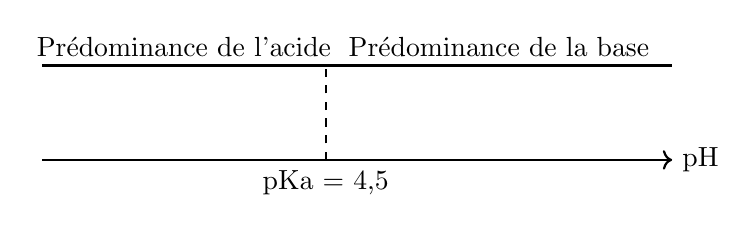
\begin{tikzpicture}[scale=0.8]
        \draw[->, thick] (0,0) -- (10,0) node[right] {pH};
        \draw[thick] (0,1.5) -- (10,1.5);
        \draw[thick, dashed] (4.5,0) node[below] {pKa = 4,5} -- (4.5,1.5);
        \node at (2.25,1.8) {Prédominance de l'acide};
        \node at (7.25,1.8) {Prédominance de la base};
    \end{tikzpicture}
    \end{center}
    }
\end{questionmult}

\begin{questionmult}{ibuprofene10}
    Déterminer la valeur du rapport des concentrations à l'équilibre de la forme acide et de la forme basique
    de l'ibuprofène dans le sang. Commenter.
    \begin{EnvQuadrillage}[NbCarreaux=20x4,Grille=Seyes,Marge=1]
    \end{EnvQuadrillage}
    \AMCOpen{}{
        \mauvaise[F]{NA}\scoring{b=0}
        \bonne[A1]{Raisonnement}\scoring{b=1}
        \bonne[A2]{Résultat}\scoring{b=1}
    }
    \explain{
    \begin{itemize}
        \item Le rapport des concentrations est donné par la relation de Henderson-Hasselbalch~:
        $$
        \frac{[\text{acide}]}{[\text{base}]} = 10^{pKa - pH}.
        $$
        \item Dans le sang (pH = 7,4), ce rapport est de $10^{4,5 - 7,4} \approx 0,0032$, ce qui signifie que la forme basique est largement prédominante.
    \end{itemize}
    }
\end{questionmult}


\AMCcleardoublepage
}

%\documentclass[12pt]{article}
\usepackage[utf8]{inputenc}
\usepackage[T1]{fontenc}
\usepackage[french]{babel}
\usepackage{amsmath}
\usepackage{WriteOnGrid}
\usepackage{siunitx}
\usepackage[version=4]{mhchem}
\usepackage{chemfig}
\usepackage[francais,bloc]{automultiplechoice}

\title{Exercice : Extraction de l'acide benzoïque}
\author{}
\date{}

\begin{document}

\maketitle

\section*{Introduction}
L'acide benzoïque, de formule \ce{C6H5COOH}, et le benzoate de sodium sont des conservateurs antimicrobiens respectivement identifiés par les codes E210 et E211. Ils sont présents dans de nombreux produits alimentaires et notamment dans certaines boissons gazeuses sucrées.

\chemfig{
OH-[:120,,1](=[:60]O)-[:180]=_[:240]-[:180]=_[:120]-[:60]=_(-[:300])
}

\section*{Données}
\begin{itemize}
    \item Masse molaire de l'acide benzoïque : $M = 122 \, \mathrm{g\cdot mol^{-1}}$.
    \item Température de fusion de l'acide benzoïque : $\theta_f = 122,4 \, \mathrm{°C}$.
    \item pKa du couple acide benzoïque/ion benzoate : $pKa = 4,2$.
    \item Le benzoate de sodium est soluble dans l’eau.
\end{itemize}

\section*{Questions}

\begin{question}{ouverte1}
Quelle est la formule topologique de l'acide benzoïque ?
\begin{EnvQuadrillage}[NbCarreaux=21x2,Grille=Seyes,Marge=1]
\end{EnvQuadrillage}
\end{question}

\begin{question}{ouverte2}
Quels sont les groupes caractéristiques présents dans la formule de l'acide benzoïque ?
\begin{EnvQuadrillage}[NbCarreaux=21x2,Grille=Seyes,Marge=1]
\end{EnvQuadrillage}
\end{question}

\begin{question}{ouverte3}
Expliquer pourquoi l'acide benzoïque est peu soluble dans l'eau mais très soluble dans l'éther éthylique.
\begin{EnvQuadrillage}[NbCarreaux=21x2,Grille=Seyes,Marge=1]
\end{EnvQuadrillage}
\end{question}

\begin{question}{ouverte4}
Écrire l'équation de la réaction de l'acide benzoïque avec l'eau.
\begin{EnvQuadrillage}[NbCarreaux=21x2,Grille=Seyes,Marge=1]
\end{EnvQuadrillage}
\end{question}

\begin{question}{ouverte5}
Quelle est l'espèce prédominante du couple acide benzoïque/ion benzoate à un pH de 3 ?
\begin{EnvQuadrillage}[NbCarreaux=21x2,Grille=Seyes,Marge=1]
\end{EnvQuadrillage}
\end{question}

\end{document}


\csvreader[head to column names]{liste.csv}{}{\sujet}

\end{document}
